% -*- latex -*-
%%%%%%%%%%%%%%%%%%%%%%%%%%%%%%%%%%%%%%%%%%%%%%%%%%%%%%%%%%%%%%%%
%%%%%%%%%%%%%%%%%%%%%%%%%%%%%%%%%%%%%%%%%%%%%%%%%%%%%%%%%%%%%%%%
%%%%
%%%% This text file is part of the source of 
%%%% `The Art of HPC, vol 4: HPC Carpentry'
%%%% by Victor Eijkhout, copyright 2012-2022
%%%%
%%%% This book is distributed under a Creative Commons Attribution 3.0
%%%% Unported (CC BY 3.0) license and made possible by funding from
%%%% The Saylor Foundation \url{http://www.saylor.org}.
%%%%
%%%%
%%%%%%%%%%%%%%%%%%%%%%%%%%%%%%%%%%%%%%%%%%%%%%%%%%%%%%%%%%%%%%%%
%%%%%%%%%%%%%%%%%%%%%%%%%%%%%%%%%%%%%%%%%%%%%%%%%%%%%%%%%%%%%%%%

Much of the teaching in this book is geared towards enabling you to
write fast code, whether this is through the choice of the right
method, or through optimal coding of a method. Consequently, you
sometimes want to measure just \emph{how fast} your code is. If you
have a simulation that runs for many hours, you'd think just looking
on the clock would be enough measurement. However, as you wonder
whether your code could be faster than it is, you need more detailed
measurements. This tutorial will teach you some ways to measure the
behavior of your code in more or less detail.

Here we will discuss 
\begin{itemize}
\item timers: ways of measuring the execution time (and sometimes
  other measurements) of a particular piece of code, and
\item profiling tools: ways of measuring how much time each piece of
  code, typically a subroutine, takes during a specific run.
\end{itemize}

\Level 0 {Timers}
\label{sec:perf-timers}
\index{timer|(}

There are various ways of timing your code, but mostly they come down
to calling a \emph{timer} routine twice that tells you the clock values:
\begin{verbatim}
  tstart = clockticks()
  ....
  tend = clockticks()
  runtime = (tend-tstart)/ticks_per_sec
\end{verbatim}

Many systems have their own timers:
\begin{itemize}
\item MPI see section~\PCSEref{sec:mpi-timing};
\item OpenMP see section~\PCSEref{sec:omp-timing};
\item PETSc see section~\PCSEref{sec:petsc-timing}.
\end{itemize}

\Level 1 {Fortran}
\index{timer!routines, Fortran}

For instance, in \emph{Fortran} there is the \n{system_clock}
routine\index{systemclock@\n{system_clock}}:
\verbatiminput{code/papi/timers/ftimer.F}
with output
\begin{verbatim}
 Clock frequency:       10000
   1.000000       813802544   813826097   2.000000  
\end{verbatim}

\Level 1 {C}
\index{timer!routines, C}

In \emph{C} there is the \n{clock} function:
\verbatiminput{papi/timers/ctimer.c}
with output
\begin{verbatim}
clock resolution: 1000000
res: 1.000000e+00
start/stop: 0.000000e+00,2.310000e+00
Time: 2.310000e+00
\end{verbatim}
Do you see a difference between the Fortran and C approaches? Hint:
what happens in both cases when the execution time becomes long? At
what point do you run into trouble?

\Level 1 {C++}
\index{timer!routines, C++}

While C routines are available in~\emph{C++}, there is also a new
\indextermtt{chrono} library that can do many things, including
handling different time formats.
\begin{verbatim}
std::chrono::system_clock::time_point start_time;
start_time = std::chrono::system_clock::now();
// ... code ...
auto duration =
    std::chrono::system_clock::now()-start_time;
auto millisec_duration =
    std::chrono::duration_cast<std::chrono::milliseconds>(duration);
std::cout << "Time in milli seconds: " 
          << .001 * millisec_duration.count() << endl;
\end{verbatim}
For more details, see \ISPref{sec:chrono}.

\Level 1 {System utilities}

There are unix system calls that can be used for timing:
\indextermtt{getrusage}
\begin{verbatim}
#include <sys/resource.h>                        
double time00(void)                              
{                                                
   struct rusage ruse;
   getrusage(RUSAGE_SELF, &ruse);
   return( (double)(ruse.ru_utime.tv_sec+ruse.ru_utime.tv_usec
    / 1000000.0) );
}
\end{verbatim}
and \indextermtt{gettimeofday}
\begin{verbatim}
#include <sys/time.h>
double time00(void)
{
   struct timeval tp;
   gettimeofday(&tp, NULL);
   return( (double) (tp.tv_sec + tp.tv_usec/1000000.0) ); /* wall
}
\end{verbatim}
These timers have the advantage that they can
distinguish between user time and system time, that is, exclusively
timing program execution or giving \indexterm{wallclock time}
including all system activities.

\index{timer|)}

\Level 0 {Accurate counters}

The timers in the previous section had a resolution of at best a
millisecond, which corresponds to several thousand cycles on a modern
CPU. For more accurate counting it is typically necessary to use
assembly language, such as the Intel \indexterm{RDTSC} (ReaD Time Stamp
Counter)
instruction~\url{http://developer.intel.com/drg/pentiumII/appnotes/RDTSCPM1.HTM}.
\begin{verbatim}
static inline void microtime(unsigned *lo, unsigned *hi)
{
  __asm __volatile (
        ".byte 0x0f; .byte 0x31   # RDTSC instruction
         movl    %%edx,%0          # High order 32 bits
         movl    %%eax,%1          # Low order 32 bits"
                 : "=g" (*hi), "=g" (*lo) :: "eax", "edx");
}                                                
\end{verbatim}
However,
this approach of using processor-specific timers is not portable. For
this reason, the \indexterm{PAPI} package (\url{http://icl.cs.utk.edu/papi/})
provides a uniform interface to \indexterm{hardware counters}.
You can see this package in action in the codes in
appendix~\HPSCref{app:codes}.

In addition to timing, hardware counters can give you information about 
such things as cache misses and instruction counters. A~processor typically
has only a limited number of counters, but they can be assigned to various tasks.
Additionally, PAPI has the concept of \emph{derived metrics}.

\Level 0 {Parallel timers in MPI and OpenMP}

Many packages have their own timers. For instance for
\emph{MPI}\index{MPI!timer}\index{timer!MPI}
\begin{lstlisting}
double MPI_Wtime(void);
double MPI_Wtick(void);
\end{lstlisting}
See \PCSEref{sec:mpi-timing}.

For
\emph{OpenMP}\index{OpenMP!timer}\index{timer!OpenMP}
\begin{lstlisting}
double omp_get_wtime()
double omp_get_wtick()
\end{lstlisting}
See \PCSEref{sec:omp-timing}.

In neither of these packages are the timers
likely to be synchronized over the
parallel processes or threads.
This means that the timings of one code segment may be widely different
on two processes/threads/tasks.
To have a synchronized timer you need
to use an explicit barrier:
\begin{lstlisting}
Barrier();
tstart = Wtime();
Barrier();
duration = Wtime()-tstart;
\end{lstlisting}

\Level 0 {Profiling tools}

Profiling tools will give you the time spent in various events in the
program, typically functions and subroutines, or parts of the code
that you have declared as such. The tool will then report how many
time the event occurred, total and average time spent, et cetera.

The only tool we mention here is \indexterm{gprof}, the profiler of
the \indexterm{GNU} compiler.
The TAU tool, discussed in section~\ref{tut:tau} for the purposes of tracing,
also has profiling capabilities, presented in a nice graphic way.
Finally, we mention that the \indexterm{PETSc} library
allows you to define your own timers and events.

\begin{verbatim}
% gcc  -g -pg ./srcFile.
% gprof    ./exeFile gmon.out > profile.txt
% gprof -l ./exeFile gmon.out > profile_line.txt
% gprof -A ./exeFile gmon.out > profile_anotated.tx
\end{verbatim}

\Level 1 {MPI profiling}

The MPI library has been designed to make it easy to profile.
See \PCSEref{sec:mpi-performance}.

\Level 0 {Tracing}

In profiling we are only concerned with aggregate information: how
many times a routine was called, and with what total/average/min/max
runtime. However sometimes we want to know about the exact timing of
events. This is especially relevant in a parallel context when we care
about \indextermbus{load}{unbalance} and \indexterm{idle time}.

Tools such as Vampyr can collect trace information about
events and in particular messages, and render them in displays such as
figure~\ref{fig:vampyr}.
\begin{figure}[ht]
  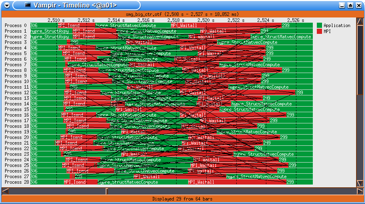
\includegraphics{vampyrtrace}
  \caption{A Vampyr timeline diagram of a parallel process.}
  \label{fig:vampyr}
\end{figure}

%% \TUTORIAL{Timing, tracing}{tracing}

\Level 0 {Parallel timing}

Timing parallel operations is fraught with peril,
as processes or threads can interact with each other.
This means that you may be measuring the wait time
induced by synchronization.
Sometimes that is actually what you want,
as in the case of a \indexterm{ping-pong} operation;
section~\PCSEref{sec:mpi-send-recv}.

Other times, this is not what you want.
Consider the code
\begin{lstlisting}
if (procno==0)
  do_big_setup();
t = timer();
mpi_some_collective();
duration = timer() - t;
\end{lstlisting}

\begin{figure}[ht]
  \hbox\bgroup
  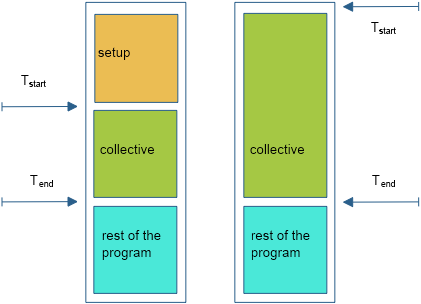
\includegraphics[scale=.5]{timenobarrier}
  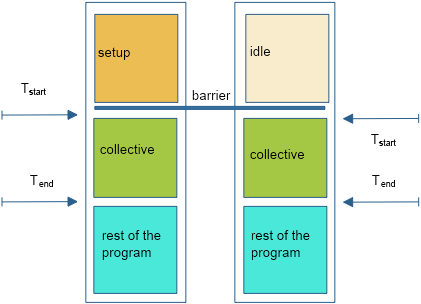
\includegraphics[scale=.5]{timebarrier}
  \egroup
  \caption{Timing a parallel code without and with barrier}
  \label{fig:time-collective}
\end{figure}

Figure~\ref{fig:time-collective} illustrates this:
\begin{itemize}
\item in the naive scenario, processes other than zero start the collective immediately,
  but process zero first does the setup;
\item all processes presumably finish more or less together.
\end{itemize}
On the non-zero processes we now get a time measurement,
which we intended to be just the collective operation,
that includes the setup time of process zero.

The solution is to put a barrier around the section that you want to time;
see again figure~\ref{fig:time-collective}.


% LocalWords:  Eijkhout systemclock chrono unix getrusage wallclock
% LocalWords:  gettimeofday RDTSC ReaD PAPI MPI OpenMP gprof PETSc cc
% LocalWords:  PMPI Vampyr timeline TACC sh cxx jumpshot
